\documentclass[]{paper}
\usepackage{amsmath}
\usepackage{amssymb}
\usepackage{float}
\usepackage{tabularx}

\newcommand{\keep}{\textsc{keep}}
\newcommand{\edit}{\textsc{edit}}
\newcommand{\drop}{\textsc{drop}}
\newcommand{\stale}[1]{\textbf{#1}}

\begin{document}

\title{DiffusEdit: Synthetic Training Data against FRUIT}

\author[*]{Tatva Agarwal}
\author[*]{Vedant Kulkarni}
\author[*]{Byasani Vedavyas}
\author[*]{Venya Velmurugan}

\affiliation[]{IIIT Hyderabad}

\contribution[*]{Equal contribution; authors listed alphabetically.}

\abstract{
In the progress report, heads trained on FRUIT-Wiki labels read little from frozen LLaDA-8B hidden states. The sentence classifier reached macro-F1 0.499 and the token staleness head AUROC 0.645, and the head's masks made infilling worse than the unchanged sentence. FRUIT labels are noisy, and only 17\% of its edits are supported by the evidence, so those numbers do not separate a weak method from weak supervision. This report repeats the same pipeline, with the same scripts, model and settings, on a synthetic train set of 9,183 articles whose labels are exact and whose evidence states every change. On it the block-24 classifier reaches macro-F1 0.870 and the staleness head AUROC 0.993, while a sentence-encoder baseline stays at its FRUIT level (0.443 against 0.433). Infilling with the head's masks now beats the unchanged sentence by 0.058 ROUGE-L and writes 61.0\% of the entities the update adds, both at Holm-corrected $p = 0.003$, and it trails infilling with the true masks by 0.014 ROUGE-L. The frozen states therefore do carry the comparison between article and evidence, and the FRUIT scores are bounded by the data. The synthetic edits are entity swaps, many of them implausible in context, so the size of the gain overstates what a harder set would show. No model trained here has been evaluated on FRUIT.
}

\date{October 14, 2026}
\correspondence{\email{vedant.kulkarni@students.iiit.ac.in}}

\maketitle{}

\section{Introduction}
\label{sec:intro}

DiffusEdit edits an outdated article in place. A sentence classifier labels each sentence \keep{}, \edit{} or \drop{}, a token staleness head chooses the tokens of an \edit{} sentence to mask, and a frozen masked diffusion model, LLaDA-8B \citep{nie-etal-2025-llada}, infills the masks from the evidence. Both heads are single linear layers on the frozen model's hidden states.

The progress report trained the heads on FRUIT-Wiki \citep{iv-etal-2022-fruit}, where the labels come from an automatic alignment of two Wikipedia snapshots. The classifier reached macro-F1 0.499 and the staleness head AUROC 0.645, and two explanations fit these scores equally. Either the frozen states do not hold the information the heads need, or they hold it and the FRUIT supervision is too noisy and too poorly supported to expose it. A train set with exact labels and complete evidence separates the two. If the heads still fail on it, the method is at fault. If they succeed, the data bounds the FRUIT scores.

This report runs that control. It answers four questions.

\begin{enumerate}
\item How does the synthetic train set differ from FRUIT, and can a model solve it from surface patterns alone?
\item With exact labels, how well do the same heads find the sentences and tokens that need to change?
\item Does infilling with predicted masks now improve on the unchanged sentence?
\item Which FRUIT findings carry over, and which reverse?
\end{enumerate}

\Cref{sec:data} describes the two train sets. \Cref{sec:setup} covers the runs. \Cref{sec:classifier,sec:staleness,sec:infilling} report the three components side by side, \Cref{sec:tests} gives the significance tests, \Cref{sec:examples} shows examples, and \Cref{sec:findings} lists the findings, the limitations and the next steps. The measures and tests are those of the progress report (its Section~2) and are not defined again here. FRUIT is blue and the synthetic set is orange in every figure.

\section{Data}
\label{sec:data}

\subsection{FRUIT}

The FRUIT train set of the progress report has 84,117 articles and 384,788 source sentences. A greedy sentence aligner derives the labels, and a word-level diff marks the stale tokens. A hand review of the 111 most disputed sentences found 21.6\% of the labels wrong. An \edit{} sentence is \emph{supported} when every word its gold rewrite adds appears in the source sentence or in the article's evidence.

\subsection{The Synthetic Set}

The synthetic set starts from sentences of Wikipedia articles, which serve as gold text. Each article is built in two steps.

\paragraph{Corruption.} The script \texttt{datasets/synthetic/rebuild.py} produces the outdated article from the gold one. The spaCy model \texttt{en\_core\_web\_sm} 3.8.0 tags the entities of each sentence, with the 13 types of the FRUIT mention extractor. For an \edit{} sentence, one to three entities (with probabilities 0.6, 0.3 and 0.1) are replaced by an entity of the same type, the same word count and the same use of digits, drawn from the other articles. A year moves by 1 to 15 years, and an integer becomes another integer of the same length. The replaced spans are the stale spans, so the token labels are exact by construction. A \drop{} sentence is a gold sentence that the target article omits. A sentence without an entity stays \keep{}.

\paragraph{Evidence.} Language model agents (Claude Sonnet~5.5) wrote the evidence, 100 articles per agent, under the instructions in \texttt{datasets/synthetic/prompt.md}. Each passage reads as an excerpt of another document, such as an encyclopedia article, a news clipping or a press release, and carries that document's title. For an \edit{} sentence a passage states the correct fact and contains the gold text of every stale span. For a \drop{} sentence a passage gives a concrete reason why the sentence no longer holds. About half of the \keep{} sentences get a consistent passage, so the presence of a related passage does not signal a change, and about one article in three gets a background passage that bears on no sentence. No passage may copy seven or more consecutive words of a sentence or contain the text of a stale span.

The script \texttt{datasets/synthetic/merge.py} enforces these rules and keeps an article only if every check passes. Of 10,000 articles written, 9,183 pass. 745 fail the copy rule, 70 lack the gold text of a span, and 2 contain stale text. A pilot with a smaller writer model (Claude Haiku~4.5) passed 8 of 100 articles, against 93 of 100 for the model used.

\subsection{Comparison}

\Cref{tab:data} and \Cref{fig:data} compare the synthetic set with a random sample of FRUIT of the same size. Three differences affect the later sections. \drop{} is rare in the synthetic set (2.8\% of sentences against 13.0\%). Its \edit{} sentences change less text, a mean of 15.6\% of the characters against 26.7\%. And 99.9\% of its \edit{} sentences with new words are supported, against 17.2\% on FRUIT.

\begin{table}[t]
\caption{The synthetic train set and a random sample of the FRUIT train set of the same number of articles (seed 42).}
\label{tab:data}
\centering
\footnotesize
\begin{tabular}{lrr}
\toprule
 & FRUIT sample & Synthetic \\
\midrule
Articles & 9,183 & 9,183 \\
Sentences & 42,219 & 31,315 \\
\quad\keep{} & 19,019 (45.0\%) & 18,628 (59.5\%) \\
\quad\edit{} & 17,718 (42.0\%) & 11,813 (37.7\%) \\
\quad\drop{} & 5,482 (13.0\%) & 874 (2.8\%) \\
Sentences per article & 4.60 & 3.41 \\
Evidence passages per article & 6.12 & 2.18 \\
Mean stale share of an \edit{} sentence's characters & 26.7\% & 15.6\% \\
\edit{} sentences with new words that are supported & 17.2\% & 99.9\% \\
Label source & aligner (silver) & construction (exact) \\
\bottomrule
\end{tabular}
\end{table}

\begin{figure}[t]
\centering
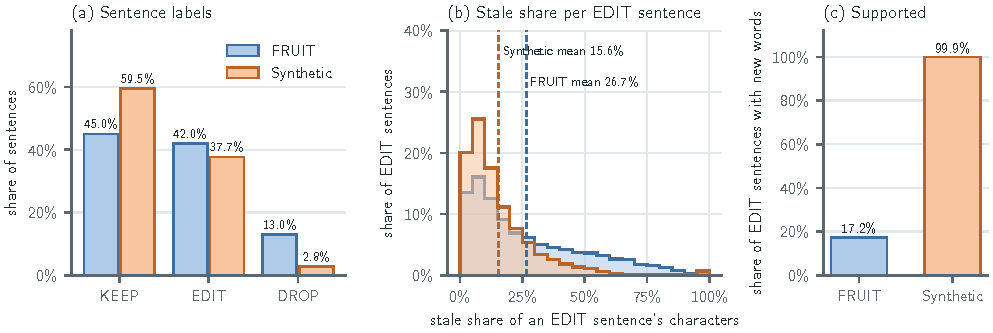
\includegraphics[width=\linewidth]{figures/data.pdf}
\caption{The two train sets. (a)~Share of sentences per label. (b)~Distribution of the stale share of characters over \edit{} sentences, with the mean of each set as a dashed line. (c)~Share of \edit{} sentences with new words whose new words all appear in the source sentence or the evidence.}
\label{fig:data}
\end{figure}

\subsection{Shortcut Probe}

A synthetic set can leak its labels through its form, for example through a fixed phrase in the evidence of every \drop{} sentence. A \emph{shortcut probe} measures this. The probe is a linear classifier that does not read the text for meaning. It sees a bag of the words and word pairs of the sentence, and eight flags that describe string matches between the sentence and the evidence, such as whether the sentence appears inside a passage. The script \texttt{datasets/synthetic/probe.py} trains it on 90\% of the articles and reports macro-F1 on the rest.

\Cref{fig:probe} gives the result. With all features the probe reaches macro-F1 0.418 on the synthetic set and 0.437 on the FRUIT sample, against 0.333 for a uniform guess. Its \drop{} F1 on the synthetic set is 0.034. Surface form therefore predicts the synthetic labels no better than it predicts the FRUIT labels, and any score well above 0.42 in \Cref{sec:classifier} needs the content of the evidence.

\begin{figure}[t]
\centering
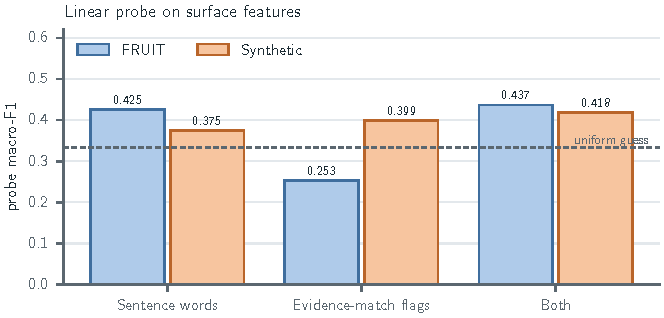
\includegraphics[width=0.66\linewidth]{figures/probe.pdf}
\caption{Macro-F1 of a linear probe on surface features, on 10\% of each set held out from the probe. Sentence words are the words and word pairs of the sentence alone. Evidence-match flags describe string matches between the sentence and the evidence.}
\label{fig:probe}
\end{figure}

\section{Setup}
\label{sec:setup}

The synthetic runs use the scripts, the model revision (LLaDA-8B-Base at \texttt{0f2787f}, bf16) and the settings of the FRUIT runs, on the same A100 with 40~GB of memory. One script, \texttt{jobs/jl/run\_synthetic.sh}, runs every stage of the three FRUIT scripts and writes to a separate directory. All stages finished in 34 minutes with no failure. Feature extraction took 5 minutes 43 seconds (31.5 articles per second) and produced no non-finite values. It stored 31,315 sentence vectors, 19,991 passage vectors and 347,903 token states.

Every head holds out 10\% of the articles with the split function and seed of the FRUIT runs. With seed 42 the held-out set has 3,116 sentences (1,838 \keep{}, 1,194 \edit{}, 84 \drop{}) and 34,049 tokens of \edit{} sentences. The FRUIT held-out set has 38,267 sentences and 531,706 tokens. The infilling runs use the first 50 of the 659 held-out articles that contain a supported \edit{} sentence.

Two evaluation scripts read fields that only FRUIT records have. \texttt{infilling/entities.py} and \texttt{infilling/significance.py} now take the gold rewrite through one function that reads either schema. The analyses of \Cref{sec:infilling,sec:tests} and all figures run on saved outputs without the GPU (\texttt{analysis/synthetic.py}).

\section{Sentence Classifier}
\label{sec:classifier}

\subsection{Results}

\Cref{tab:classifier} and \Cref{fig:classifier} report the held-out scores. On the synthetic set the block-24 classifier reaches macro-F1 0.870, against 0.499 on FRUIT. The MiniLM baseline, which embeds the sentence and the mean of the passages without LLaDA, scores 0.443, within 0.010 of its FRUIT score and within 0.025 of the shortcut probe. The gain is therefore specific to the LLaDA states of the pass that reads the evidence before the article.

\begin{table}[t]
\caption{Sentence classifier on the held-out set with seed 42, and macro-F1 as mean $\pm$ standard deviation over five seeds. The synthetic held-out set has 3,116 sentences and the FRUIT one 38,267.}
\label{tab:classifier}
\centering
\footnotesize
\setlength{\tabcolsep}{4pt}
\begin{tabular}{llccccc}
\toprule
Train set & Model & Macro-F1 & \keep{} F1 & \edit{} F1 & \drop{} F1 & 5 seeds \\
\midrule
FRUIT & MiniLM baseline & 0.433 & 0.440 & 0.580 & 0.278 & $0.436 \pm 0.003$ \\
 & LLaDA block 24, cross-entropy & \textbf{0.499} & 0.558 & 0.626 & 0.315 & $0.499 \pm 0.002$ \\
 & LLaDA block 32, cross-entropy & 0.490 & 0.534 & 0.611 & 0.327 & $0.490 \pm 0.002$ \\
 & LLaDA block 24, focal & 0.490 & 0.549 & 0.608 & 0.312 & $0.490 \pm 0.002$ \\
\midrule
Synthetic & MiniLM baseline & 0.443 & 0.563 & 0.564 & 0.201 & $0.443 \pm 0.018$ \\
 & LLaDA block 24, cross-entropy & \textbf{0.870} & 0.946 & 0.921 & 0.742 & $0.849 \pm 0.015$ \\
 & LLaDA block 32, cross-entropy & 0.708 & 0.871 & 0.833 & 0.419 & $0.691 \pm 0.010$ \\
 & LLaDA block 24, focal & 0.853 & 0.950 & 0.934 & 0.674 & $0.839 \pm 0.012$ \\
\bottomrule
\end{tabular}
\end{table}

\begin{figure}[t]
\centering
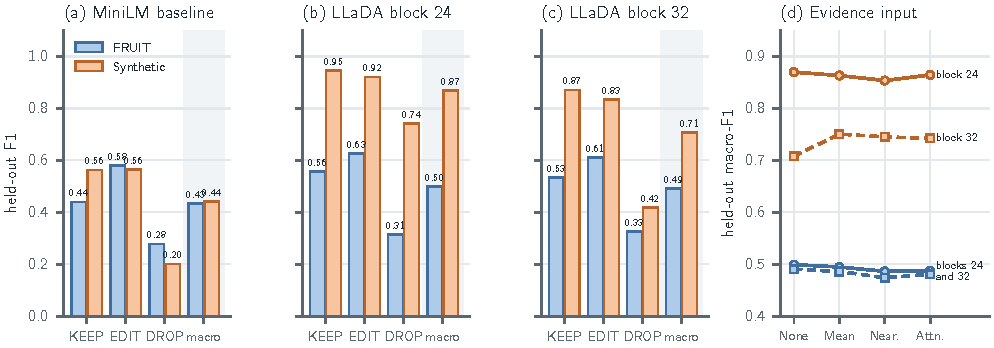
\includegraphics[width=\linewidth]{figures/classifier.pdf}
\caption{Sentence classifier on the held-out sets, seed 42. (a) to (c)~Per-class F1 and macro-F1 of the baseline and of LLaDA at blocks 24 and 32, using the sentence vector alone. (d)~Macro-F1 when an evidence vector joins the LLaDA sentence vector. The y axis of panel (d) starts at 0.4.}
\label{fig:classifier}
\end{figure}

\subsection{Depth}

Block 24 exceeds block 32 by 0.162 macro-F1 on the synthetic set. On FRUIT the difference was 0.009. The final block is trained to predict tokens, and its states are closer to the output vocabulary. The comparison between a sentence and the evidence is more readable three quarters of the way up. The FRUIT runs could not show this, because the noise compressed both scores into a band of 0.01.

\subsection{Evidence Inputs}

Panel (d) of \Cref{fig:classifier} adds one evidence vector to the sentence vector. At block 24 the three variants change macro-F1 by $-0.006$ to $-0.016$, within the seed spread of 0.015, as on FRUIT. At block 32 they add 0.034 to 0.043, where on FRUIT they lowered the score. The block-24 sentence vector already encodes what the evidence says about the sentence, so a separate evidence vector adds nothing. The block-32 vector has lost part of it.

\subsection{Errors}

\Cref{fig:confusion} shows the confusion matrices at block 24. On FRUIT every off-diagonal cell holds at least 16\% of its row. On the synthetic set \keep{} and \edit{} are recognised in 93\% and 95\% of cases. \drop{} is the weak class at 70\% (59 of 84), and its errors go to \edit{} (18) more than to \keep{} (7). The classifier detects that the evidence contradicts the sentence and then mistakes a contradiction that removes the sentence for one that corrects it.

\begin{figure}[t]
\centering
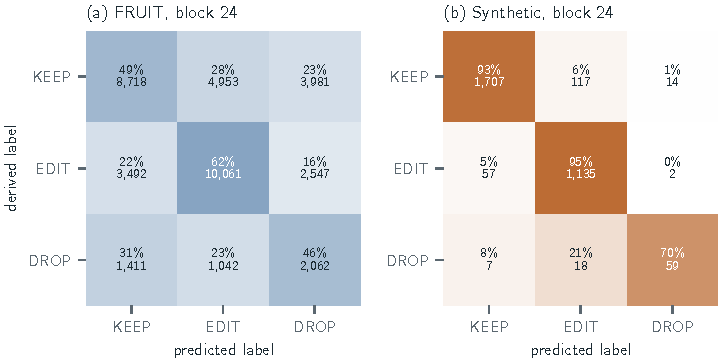
\includegraphics[width=0.74\linewidth]{figures/confusion.pdf}
\caption{Confusion matrices of the block-24 classifier with cross-entropy on the held-out sets, seed 42. Each cell gives the share of its row and the sentence count. Rows are the labels of the data and columns the predictions after the deletion gate.}
\label{fig:confusion}
\end{figure}

\subsection{Seeds}

\Cref{fig:seeds} shows five seeds per configuration. The synthetic scores vary more across seeds (standard deviation up to 0.018 against 0.003 or less on FRUIT) because each held-out set is twelve times smaller and holds about 84 \drop{} sentences. Focal loss lowers macro-F1 on both sets, by 0.010 on average at block 24.

\begin{figure}[t]
\centering
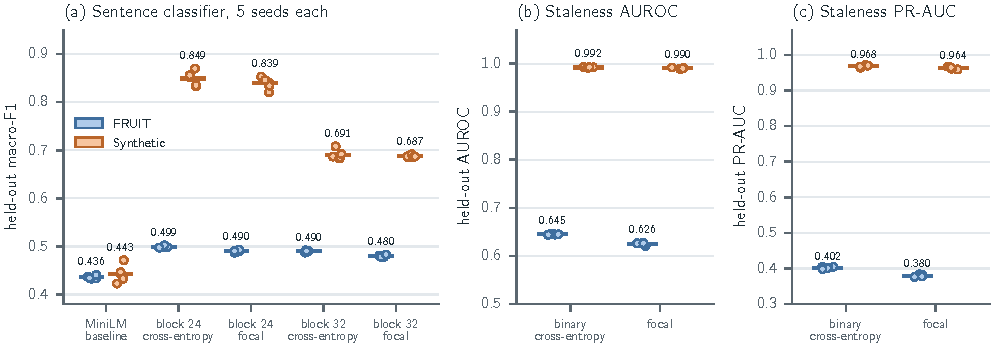
\includegraphics[width=\linewidth]{figures/seeds.pdf}
\caption{Five seeds per configuration on both train sets. Each dot is one seed with its own held-out split, bars mark the mean, and labels give the mean. (a)~Held-out macro-F1 of the sentence classifier. (b) and (c)~Held-out AUROC and PR-AUC of the staleness head.}
\label{fig:seeds}
\end{figure}

\section{Token Staleness Head}
\label{sec:staleness}

\subsection{Results}

The staleness head is one linear layer with a sigmoid on the block-32 state of each token of an \edit{} sentence. \Cref{tab:staleness} compares it on the two sets. On the synthetic set its AUROC is 0.993 and its PR-AUC 0.972, against 0.645 and 0.405 on FRUIT. At the threshold tuned for F1 it masks 14.3\% of tokens at precision 0.934 and recall 0.898. On FRUIT the tuned threshold masked 65.3\% of tokens at precision 0.344.

\begin{table}[t]
\caption{Token staleness head on the held-out tokens of \edit{} sentences, seed 42. \texttt{tau\_match} is the threshold whose masked share is closest to the stale share. The last two rows are means $\pm$ standard deviations over five seeds.}
\label{tab:staleness}
\centering
\footnotesize
\begin{tabular}{lcc}
\toprule
 & FRUIT & Synthetic \\
\midrule
Held-out tokens & 531,706 & 34,049 \\
Stale share & 28.5\% & 14.9\% \\
AUROC & 0.645 & \textbf{0.993} \\
PR-AUC & 0.405 & \textbf{0.972} \\
\midrule
Threshold tuned for F1 & 0.40 & 0.85 \\
\quad precision / recall / share masked & 0.344 / 0.789 / 65.3\% & 0.934 / 0.898 / 14.3\% \\
\texttt{tau\_match} & 0.60 & 0.80 \\
\quad precision / recall / share masked & 0.415 / 0.377 / 25.8\% & 0.915 / 0.914 / 14.9\% \\
\midrule
AUROC, binary cross-entropy, 5 seeds & $0.645 \pm 0.001$ & $0.992 \pm 0.001$ \\
AUROC, focal loss, 5 seeds & $0.626 \pm 0.003$ & $0.990 \pm 0.001$ \\
\bottomrule
\end{tabular}
\end{table}

\subsection{Scores}

\Cref{fig:stale_scores} shows why. On FRUIT the scores of stale and correct tokens form two overlapping bells centred near 0.55 and 0.45. On the synthetic set 81\% of stale tokens score above 0.96 and 66\% of correct tokens below 0.04. Panel (c) shows that neither head is calibrated. Both overstate the share of stale tokens at every score below 0.9, which is the expected effect of the positive-class weight in the loss.

\Cref{fig:stale_rules} shows the trade-off. On FRUIT precision never passes 0.65 at any recall. On the synthetic set precision stays above 0.9 up to a recall of 0.92. The masked share at the tuned threshold is now close to the stale share, so the head no longer masks most of the sentence.

\begin{figure}[t]
\centering
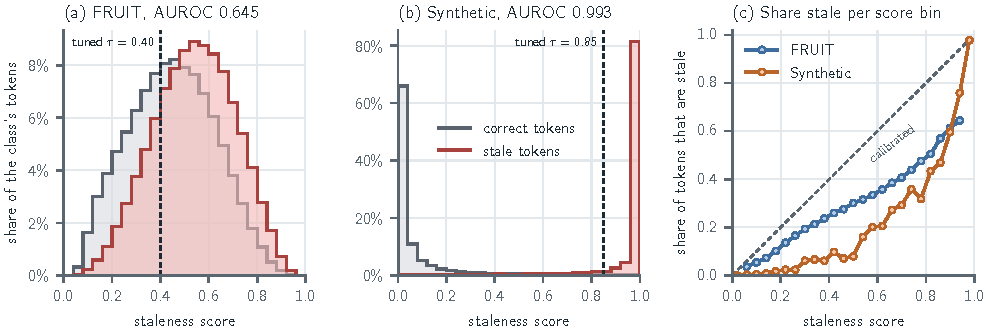
\includegraphics[width=\linewidth]{figures/stale_scores.pdf}
\caption{Staleness scores of held-out tokens, seed 42. (a) and (b)~Score distribution of stale and correct tokens on each set, each normalised to its class, with the tuned threshold as a dashed line. The y axes differ. (c)~Share of tokens that are stale per score bin, for bins with at least 50 tokens.}
\label{fig:stale_scores}
\end{figure}

\begin{figure}[t]
\centering
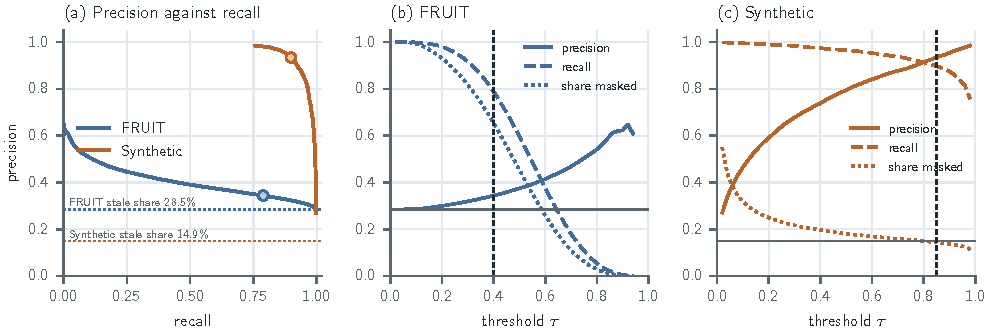
\includegraphics[width=\linewidth]{figures/stale_rules.pdf}
\caption{Threshold rules of the staleness head, seed 42. (a)~Precision against recall as the threshold moves, with the tuned threshold marked and the stale share of each set as a dotted line. (b) and (c)~Precision, recall and the share of tokens masked per threshold. The horizontal line is the stale share and the dashed vertical line the tuned threshold.}
\label{fig:stale_rules}
\end{figure}

\subsection{What the Head May Be Detecting}

Two signals could produce this separation. The head could detect that a token disagrees with the evidence, which is the intended signal. It could also detect that a token is unlikely in its context whatever the evidence says. A replacement matches the entity type that spaCy assigned, and that type is sometimes wrong, which yields sources such as ``started on Solaris 11''. The first signal transfers to real updates and the second does not. The no-evidence infilling run of \Cref{sec:infilling} shows that the frozen model alone restores the gold sentence for 18 of 99 sentences, so context carries part of the answer. A staleness head trained on states extracted without evidence would measure the share. It needs the GPU and has not been run.

\section{Infilling}
\label{sec:infilling}

\subsection{Runs}

The three runs of the progress report were repeated on 50 held-out supported articles, with 99 repaired sentences. \emph{Oracle masks} mask the stale tokens of the data. \emph{No evidence} uses the same masks and removes the evidence from the input. \emph{Predicted masks} mask the tokens that the staleness head scores at or above \texttt{tau\_match} (0.80). Sentence labels come from the data in all three, as on FRUIT. \emph{Copy} is the unchanged source sentence. A run took 13.0, 6.3 and 14.1 seconds per article, against 49.1, 13.4 and 90.9 on FRUIT, because the articles are shorter and the predicted masks cover 15.8\% of the characters and not 33.3\%.

\subsection{ROUGE-L, Hit and Coverage}

\Cref{fig:infilling} and \Cref{tab:infilling} give the results. With oracle masks ROUGE-L rises from 0.867 (copy) to 0.940. With predicted masks it reaches 0.926. On FRUIT predicted masks lowered ROUGE-L from 0.782 to 0.678. \emph{Hit}, the share of sentences where some candidate contains every new gold word, is 80.0\% with oracle masks and 77.9\% with predicted ones, against 33.3\% and 20.6\% on FRUIT. Without evidence it falls to 49.5\%.

\begin{table}[t]
\caption{Infilling on 50 held-out supported articles of each set (106 repaired sentences on FRUIT, 99 on the synthetic set). Exact match is the share of outputs equal to the gold rewrite and was computed for the synthetic set only.}
\label{tab:infilling}
\centering
\footnotesize
\setlength{\tabcolsep}{4pt}
\begin{tabular}{llcccccc}
\toprule
Train set & System & ROUGE-L & Pool ROUGE-L & Hit & Coverage & Masked & Exact match \\
\midrule
FRUIT & Copy & 0.782 & & & & & \\
 & Oracle masks & \textbf{0.801} & 0.878 & 33.3\% & 32.9\% & 24.4\% & \\
 & Oracle masks, no evidence & 0.779 & 0.861 & 21.6\% & 18.9\% & 24.4\% & \\
 & Predicted masks & 0.678 & 0.750 & 20.6\% & 15.4\% & 33.3\% & \\
\midrule
Synthetic & Copy & 0.867 & & & & & 0 of 99 \\
 & Oracle masks & \textbf{0.940} & 0.976 & 80.0\% & 79.6\% & 14.4\% & 26 of 99 \\
 & Oracle masks, no evidence & 0.905 & 0.953 & 49.5\% & 46.9\% & 14.4\% & 18 of 99 \\
 & Predicted masks & 0.926 & 0.967 & 77.9\% & 77.7\% & 15.8\% & 21 of 99 \\
\bottomrule
\end{tabular}
\end{table}

\begin{figure}[t]
\centering
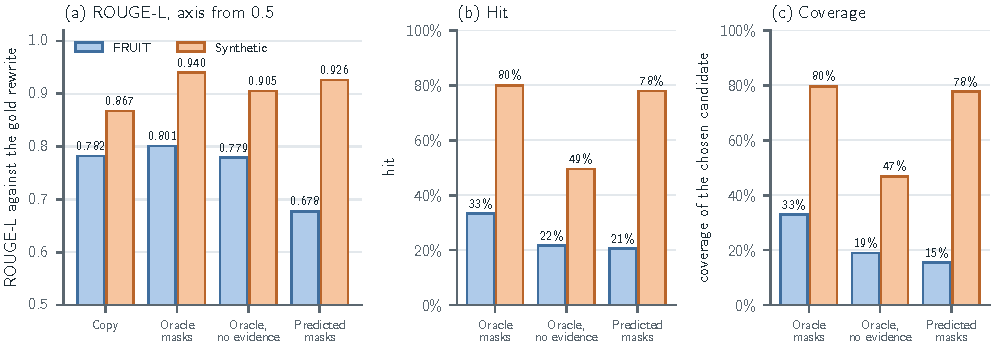
\includegraphics[width=\linewidth]{figures/infilling.pdf}
\caption{Infilling on 50 held-out supported articles of each set. (a)~ROUGE-L of the chosen candidate against the gold rewrite. The y axis starts at 0.5. (b)~Hit. (c)~Coverage, the share of new gold words in the chosen candidate.}
\label{fig:infilling}
\end{figure}

\subsection{Entity Measures}

\Cref{fig:entities} shows the five entity measures. On the synthetic set the unchanged sentence has entity precision 0.569, lower than on FRUIT (0.727), because every edit replaces an entity. Infilling with oracle masks raises it to 0.854 and removes every outdated entity (outdated kept 0.000, against 0.236 on FRUIT). New-entity recall is 0.635 with oracle masks and 0.610 with predicted masks, against 0.218 and 0.134 on FRUIT. Fabricated entities stay where they were on FRUIT, at 14.9\% with evidence and 24.2\% without. The best candidate of the pool reaches new-entity recall 0.767, so the reranker still leaves 0.132 unused, close to the 0.110 it left on FRUIT.

\begin{figure}[t]
\centering
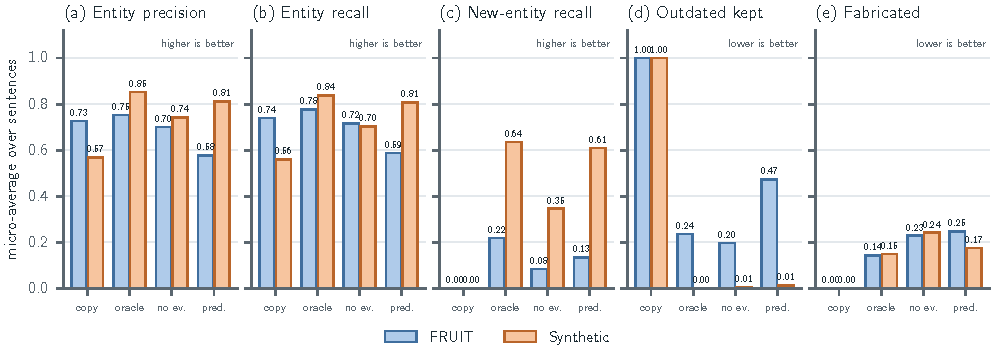
\includegraphics[width=\linewidth]{figures/entities.pdf}
\caption{Entity measures of the unchanged sentence and the three infilling systems on both sets, as micro-averages over the repaired sentences. Higher is better in panels (a) to (c) and lower in (d) and (e).}
\label{fig:entities}
\end{figure}

\section{Significance Tests}
\label{sec:tests}

\subsection{Infilling}

\Cref{tab:tests} and \Cref{fig:differences} give the paired tests between infilling systems on the synthetic set, with the article as the unit, 10,000 resamples and a Holm correction over the 30 tests of the table. The smallest attainable Holm-corrected $p$ is 0.003.

Three FRUIT results change. Oracle masks now beat the unchanged sentence on ROUGE-L by 0.072, a difference that did not survive the correction on FRUIT ($+0.019$, $p_{\text{Holm}} = 0.093$). Predicted masks beat the unchanged sentence by 0.058, where on FRUIT they lost by 0.105. And the gap between oracle and predicted masks shrinks from 0.190 entity recall to 0.030, which is not significant. The effect of evidence holds on both sets. Removing it lowers new-entity recall by 0.289 and raises fabricated entities by 0.093.

\begin{table}[t]
\caption{Paired tests between infilling systems on the synthetic set (99 sentences in 50 articles). Intervals come from a paired bootstrap and $p$-values from a paired permutation test, both over articles. Bold marks $p_{\text{Holm}} < 0.05$. The last column gives the same difference on FRUIT from the progress report, with a star where it was significant there.}
\label{tab:tests}
\centering
\footnotesize
\setlength{\tabcolsep}{4pt}
\begin{tabular}{llccccc}
\toprule
Comparison (A $-$ B) & Measure & A $-$ B & 95\% interval & $p$ & $p_{\text{Holm}}$ & FRUIT \\
\midrule
Oracle $-$ copy & ROUGE-L & $+0.072$ & $[+0.056, +0.089]$ & 0.0001 & \textbf{0.003} & $+0.019$ \\
 & Entity recall & $+0.276$ & $[+0.232, +0.331]$ & 0.0001 & \textbf{0.003} & $+0.037$ \\
 & New-entity recall & $+0.635$ & $[+0.557, +0.719]$ & 0.0001 & \textbf{0.003} & $+0.218^{*}$ \\
\midrule
Oracle $-$ no evidence & ROUGE-L & $+0.035$ & $[+0.021, +0.048]$ & 0.0001 & \textbf{0.003} & $+0.022$ \\
 & Entity recall & $+0.133$ & $[+0.091, +0.181]$ & 0.0001 & \textbf{0.003} & $+0.061^{*}$ \\
 & New-entity recall & $+0.289$ & $[+0.204, +0.383]$ & 0.0001 & \textbf{0.003} & $+0.134$ \\
 & Fabricated & $-0.093$ & $[-0.141, -0.042]$ & 0.0007 & \textbf{0.006} & $-0.085^{*}$ \\
\midrule
Predicted $-$ copy & ROUGE-L & $+0.058$ & $[+0.042, +0.075]$ & 0.0001 & \textbf{0.003} & $-0.105^{*}$ \\
 & Entity precision & $+0.242$ & $[+0.188, +0.303]$ & 0.0001 & \textbf{0.003} & $-0.149^{*}$ \\
 & Entity recall & $+0.246$ & $[+0.205, +0.294]$ & 0.0001 & \textbf{0.003} & $-0.153^{*}$ \\
 & New-entity recall & $+0.610$ & $[+0.526, +0.701]$ & 0.0001 & \textbf{0.003} & $+0.134^{*}$ \\
\midrule
Oracle $-$ predicted & ROUGE-L & $+0.014$ & $[+0.005, +0.025]$ & 0.0043 & \textbf{0.030} & $+0.124^{*}$ \\
 & Entity precision & $+0.042$ & $[+0.015, +0.072]$ & 0.0076 & \textbf{0.046} & $+0.174^{*}$ \\
 & Entity recall & $+0.030$ & $[+0.000, +0.064]$ & 0.0888 & 0.444 & $+0.190^{*}$ \\
 & New-entity recall & $+0.025$ & $[-0.028, +0.079]$ & 0.5348 & 1.000 & $+0.084$ \\
 & Fabricated & $-0.026$ & $[-0.057, +0.001]$ & 0.0938 & 0.444 & $-0.104^{*}$ \\
\bottomrule
\end{tabular}
\end{table}

\begin{figure}[t]
\centering
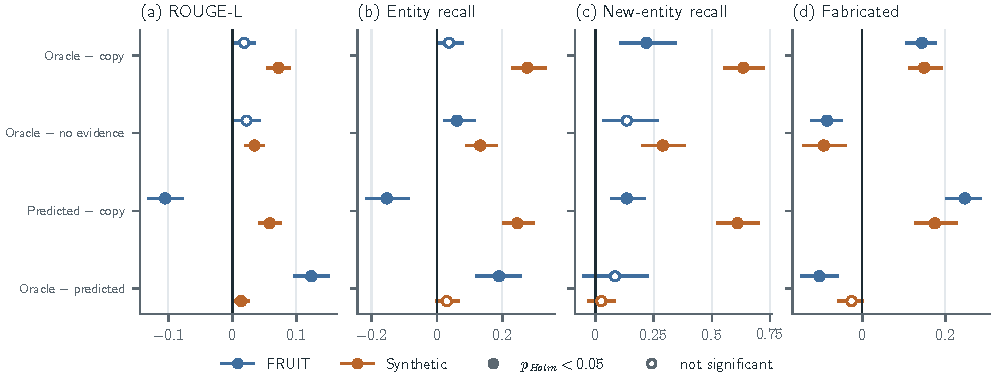
\includegraphics[width=\linewidth]{figures/differences.pdf}
\caption{Paired differences between infilling systems on both sets, with 95\% bootstrap intervals over 50 articles. A filled dot marks a Holm-corrected $p$ below 0.05. Fabricated is lower-is-better, so a negative difference favours the first system.}
\label{fig:differences}
\end{figure}

\subsection{Classifier}

\Cref{tab:classifier_tests} tests the classifier differences with the procedure of the progress report, on the 3,116 held-out sentences of seed 42 with 2,000 resamples. Block 24 exceeds the baseline by 0.427 and block 32 by 0.162, both significant, and both with the same sign on all five seeds. The difference between cross-entropy and focal loss is not significant on the synthetic set at either block. It was significant on FRUIT, where the held-out set is twelve times larger.

\begin{table}[t]
\caption{Paired tests between sentence classifiers on the synthetic held-out set, seed 42 (2,000 resamples, smallest attainable $p$ 0.0005). The last two columns give the difference on each seed's own held-out split and the seed-42 difference on FRUIT.}
\label{tab:classifier_tests}
\centering
\footnotesize
\setlength{\tabcolsep}{4pt}
\begin{tabular}{lcccccc}
\toprule
Comparison (A $-$ B) & A $-$ B & 95\% interval & $p$ & $p_{\text{Holm}}$ & 5 seeds & FRUIT \\
\midrule
Block 24 $-$ MiniLM baseline & $+0.427$ & $[+0.389, +0.463]$ & $<0.001$ & \textbf{0.002} & $+0.406 \pm 0.019$ & $+0.066$ \\
Block 24 $-$ block 32 & $+0.162$ & $[+0.124, +0.198]$ & $<0.001$ & \textbf{0.002} & $+0.158 \pm 0.010$ & $+0.009$ \\
Block 24 cross-entropy $-$ focal & $+0.017$ & $[-0.005, +0.038]$ & 0.110 & 0.120 & $+0.010 \pm 0.006$ & $+0.010$ \\
Block 32 cross-entropy $-$ focal & $+0.022$ & $[-0.004, +0.046]$ & 0.060 & 0.120 & $+0.003 \pm 0.012$ & $+0.012$ \\
\bottomrule
\end{tabular}
\end{table}

\section{Examples}
\label{sec:examples}

\Cref{tab:example_data} shows one synthetic article. \Cref{tab:example_infill} shows four repaired sentences from the infilling runs. In the first two the evidence supplies the value and both mask sources recover the gold rewrite, while the run without evidence writes a plausible wrong value. In the third the model restores the right entities and adds a word the gold rewrite lacks, which lowers exact match but not the entity measures. In the fourth the evidence names the subject only by surname, and the model invents a first name.

\begin{table}[t]
\caption{One article of the synthetic train set (\texttt{synthetic-008054}). Stale text is bold. The evidence passages follow with their titles.}
\label{tab:example_data}
\centering
\footnotesize
\begin{tabularx}{\linewidth}{lX}
\toprule
\edit{} & The football tournament at the 1976 Summer Olympics started on \stale{Solaris 11} and ended on \stale{the 1970s}. \\
\quad gold & The football tournament at the 1976 Summer Olympics started on 18 July and ended on 31 July. \\
\keep{} & Only one event, the men's tournament, was contested. \\
\edit{} & \stale{70} teams participated in the tournament, while three \stale{Kasa\"i} teams took part in the boycott. \\
\quad gold & 13 teams participated in the tournament, while three African teams took part in the boycott. \\
\midrule
Evidence & \emph{Boycott Thins Out Olympic Football Field.} A line-up of 13 sides contested the football event, after three African squads pulled out in protest. Only a men's competition was held. \\
Evidence & \emph{Montreal 1976: Football Programme.} The Olympic football event in Montreal opened on 18 July, and the gold medal match closed the competition on 31 July. \\
\bottomrule
\end{tabularx}
\end{table}

\begin{table}[t]
\caption{Four repaired sentences from the synthetic infilling runs. Stale text in the source is bold, and so is each span an output wrote in its place.}
\label{tab:example_infill}
\centering
\footnotesize
\begin{tabularx}{\linewidth}{lX}
\toprule
Source & \stale{770} -- Coronation of King Otto I of Germany. \\
Evidence & In 936 the Saxon duke Otto I was crowned king of Germany at Aachen, in the palace chapel of Charlemagne. \\
Oracle, predicted & \stale{936} -- Coronation of King Otto I of Germany. \quad (equal to the gold rewrite) \\
No evidence & \stale{962} -- Coronation of King Otto I of Germany. \\
\midrule
Source & \ldots{} is a class of bony fish that comprise \stale{about 40\%} of living vertebrate species. \\
Evidence & Ray-finned fishes, the class Actinopterygii, account for over 50\% of all vertebrate species alive today. \\
Oracle, predicted & \ldots{} comprise \stale{over 50\%} of living vertebrate species. \quad (equal to the gold rewrite) \\
No evidence & \ldots{} comprise \stale{the vast majority} of living vertebrate species. \\
\midrule
Source & \ldots{} in the old industrial area on the \stale{UK} str\"om river in the city centre of \stale{Jharkhand}. \\
Gold & \ldots{} on the Motala str\"om river in the city centre of Norrk\"oping. \\
Oracle, predicted & \ldots{} on the \stale{Motala} str\"om river in the city centre of \stale{Norrk\"oping, Sweden}. \\
No evidence & \ldots{} on the \stale{G\"ota} str\"om river in the city centre of \stale{Norrk\"oping, Sweden}. \\
\midrule
Source & \stale{Sam Clayton} ( , ; 22 February 1788 -- 21 September 1860) was a German philosopher. \\
Gold & Arthur Schopenhauer ( , ; 22 February 1788 -- 21 September 1860) was a German philosopher. \\
Evidence & Three passages, each naming him as ``Schopenhauer'' without a first name. \\
Oracle, predicted & \stale{Arturo Amiga} ( , ; 22 February 1788 -- 21 September 1860) was a German philosopher. \\
No evidence & \stale{Schopenhauer} ( , ; 22 February 1788 -- 21 September 1860) was a German philosopher. \\
\bottomrule
\end{tabularx}
\end{table}

\section{Findings and Next Steps}
\label{sec:findings}

\Cref{fig:summary} places the main measures of both sets on one axis.

\begin{figure}[t]
\centering
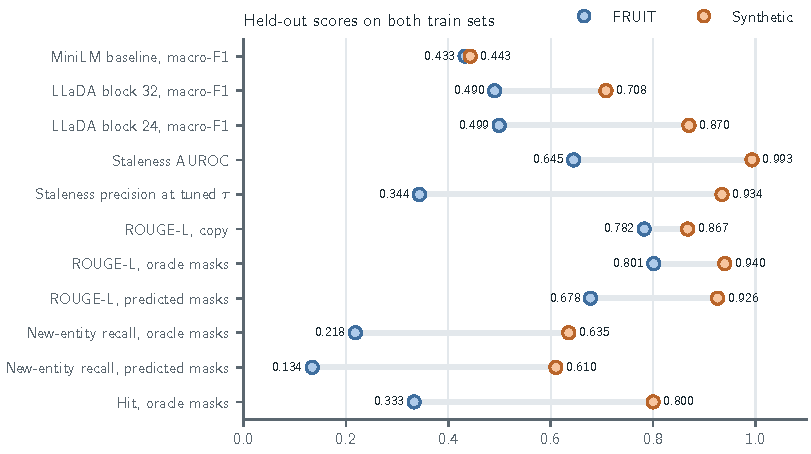
\includegraphics[width=0.82\linewidth]{figures/summary.pdf}
\caption{Held-out scores of the same pipeline trained on each set. Classifier and staleness scores are from seed 42, and infilling scores from 50 supported articles of each set.}
\label{fig:summary}
\end{figure}

\subsection{Findings}

\begin{enumerate}
\item The frozen LLaDA states hold the comparison between a sentence and the evidence. With exact labels a linear head reads it at macro-F1 0.870 for sentences and AUROC 0.993 for tokens. The FRUIT scores of 0.499 and 0.645 are bounded by the supervision.
\item The gain needs the evidence-conditioned LLaDA pass. A sentence encoder with a mean evidence vector scores 0.443, near the 0.418 of a probe on surface features and near its own FRUIT score.
\item Block 24 is the better layer for sentence labels by 0.162 macro-F1. On FRUIT the two blocks were 0.009 apart.
\item A separate evidence vector does not help at block 24 on either set. It helps at block 32 on the synthetic set only.
\item The staleness head no longer limits the system. Infilling with its masks beats the unchanged sentence on every measure and trails oracle masks by 0.014 ROUGE-L. On FRUIT its masks made the output worse than the unchanged sentence.
\item Evidence changes the output on both sets. Removing it costs 0.289 new-entity recall and adds 0.093 fabricated entities on the synthetic set.
\item Two FRUIT results carry over unchanged. About 15\% of output entities are fabricated even with oracle masks and evidence, and the candidate pool holds outputs with 0.13 more new-entity recall than the reranker picks.
\item \drop{} remains the weakest class. One in five \drop{} sentences is labelled \edit{}.
\end{enumerate}

\subsection{Limitations}

The synthetic task is easier than FRUIT in ways that this report does not separate from label quality. Every edit is an entity swap, the corrected value appears verbatim in a passage, and a swap is often implausible in its context. \Cref{sec:staleness} explains why the last point may inflate the staleness scores. The reasons that the \drop{} passages give are invented, because the dropped sentences are true Wikipedia sentences. The train set has 9,183 articles, 11\% of FRUIT, and 874 \drop{} sentences, so the held-out \drop{} score rests on 84 sentences. Some source sentences are fragments left by a sentence splitter that breaks at abbreviations. The infilling runs use 50 articles, one round and the sentence labels of the data. The per-sentence masking rules of the progress report were not recomputed, because the saved token scores do not record which sentence a token belongs to. No model trained on the synthetic set has been evaluated on FRUIT, so nothing here shows transfer.

\subsection{Next Steps}

\begin{enumerate}
\item \emph{Staleness without evidence.} Extract states without the evidence and train the staleness head on them. Its AUROC is the share of the 0.993 that comes from implausible swaps. This needs one extraction pass of about six minutes.
\item \emph{Transfer.} Apply the synthetic heads to the FRUIT held-out features, and train on the union of both sets. The FRUIT features are on the instance.
\item \emph{Harder corruptions.} Draw each replacement from entities of the same article or of a related one, so that it is plausible in context, and add edits that are not entity swaps.
\item \emph{More \drop{} sentences.} Raise the share of \drop{} towards the 13\% of FRUIT, and write passages for the 20,000 corrupted articles that have none.
\item \emph{Classifier into infilling.} Feed the predicted sentence labels to infilling and measure the end-to-end system. All runs so far take the sentence labels from the data.
\item \emph{Reranker.} The entity-aware term proposed in the progress report applies unchanged, since the pool gap is the same on both sets.
\end{enumerate}

\clearpage
\bibliographystyle{plainnat}
\bibliography{../../paper/paper,../../progress/progress}

\end{document}
